\section{Methodology}

This section describes the systematic evaluation of the architectural design implemented for the Plant Up! ecosystem. While the overarching theme of this thesis contrasts Edge versus Cloud processing, the objective of these experiments is to empirically validate the feasibility and optimizations of the core backend infrastructure that makes the \textit{Thin Edge} viable. Controlled benchmarks were conducted focusing on ingestion latency, time‑series retrieval efficiency, and middleware resilience under peak network influx.

\subsection{Experimental Control Framework}
The experimental framework targets the core cloud‑centric components. Physical ESP32 devices act solely as telemetry ingress vectors, while a C\# Middleware Gateway buffers MQTT messages and performs batch inserts into a Supabase‑managed PostgreSQL instance with TimescaleDB extensions. The primary configuration under test implements a hybrid \textit{Thin Edge} paradigm: ESP32 devices generate raw JSON payloads without local decision‑making, and all processing is performed in the cloud.

\begin{figure}[H]
    \centering
    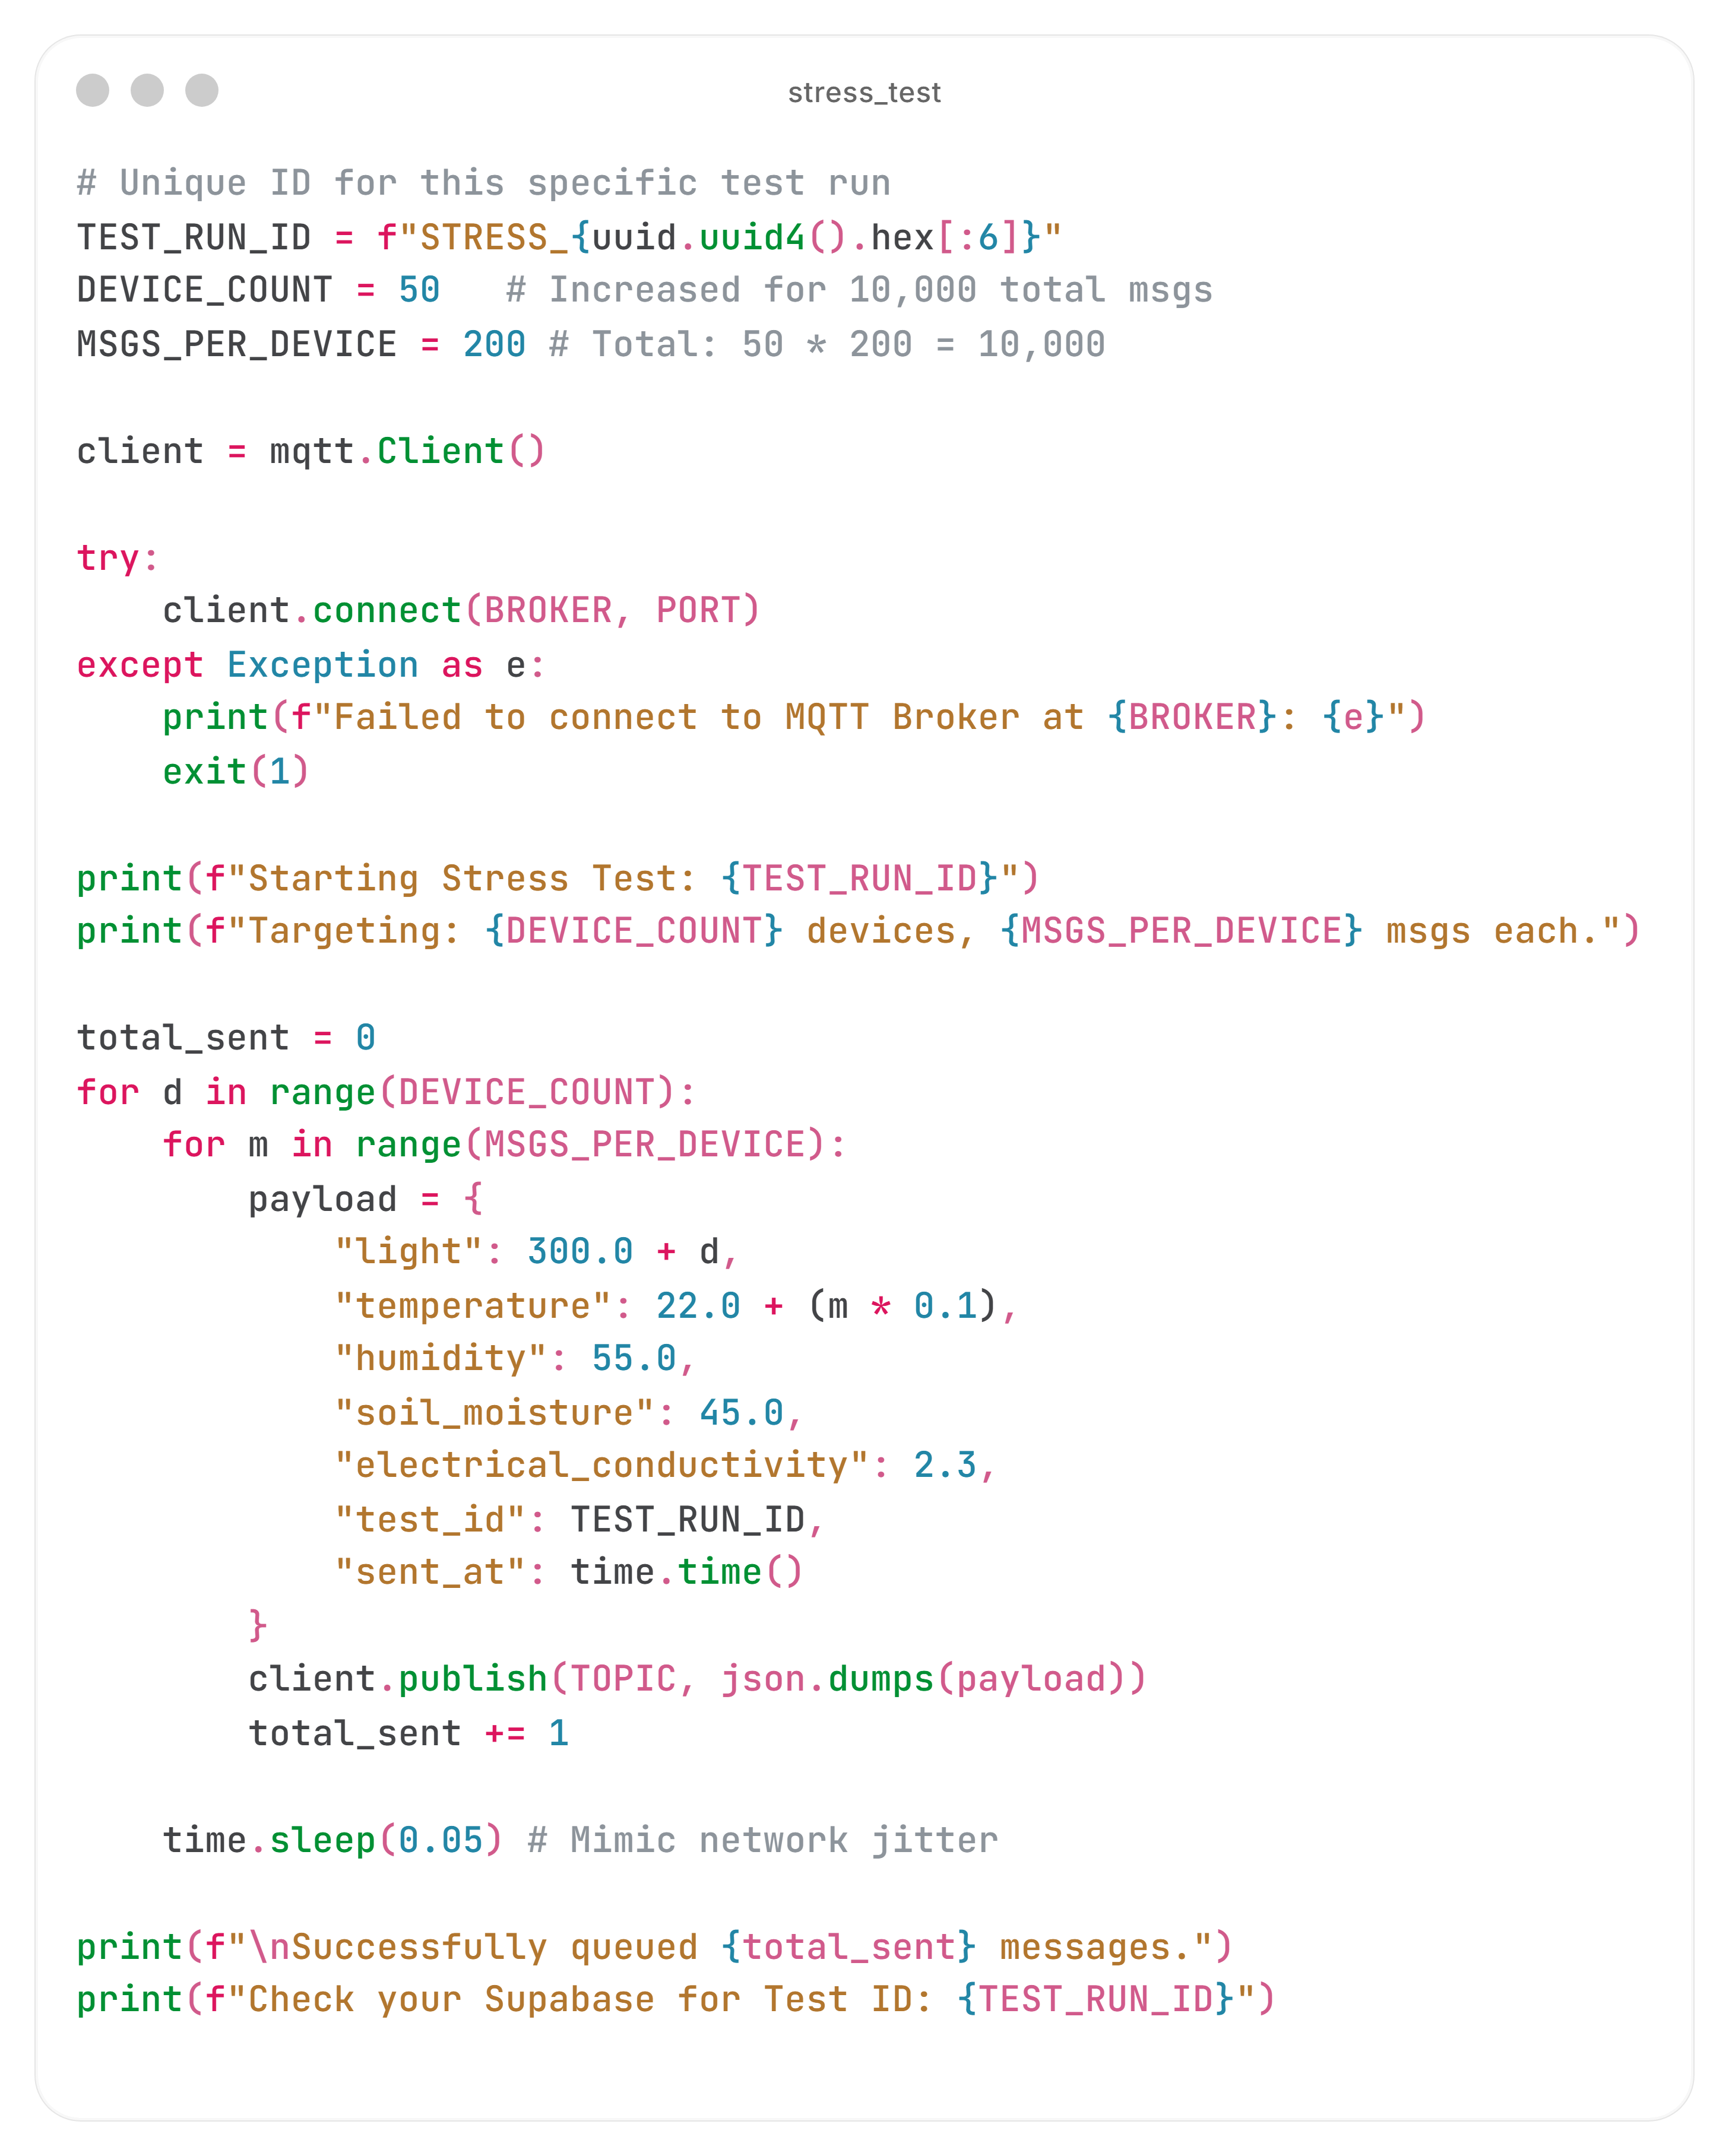
\includegraphics[width=0.8\textwidth]{Abudi/figures/stress_test.png}
    \caption{Benchmark runner (Python)}
    \label{fig:benchmark_python}
\end{figure}

\subsection{Measurement Methodology and Environment}
\begin{figure}[H]
    \centering
    \scalebox{1.1}{\IoTNavigator{1}{0}{2}}
    \caption{Data‑pipeline layers involved in the stress‑test scenario.}
\end{figure}
The testing environment consists of a Supabase cloud backend with a dedicated PostgreSQL instance. Load generation is performed by the Python simulation above using the \texttt{paho‑mqtt} library, allowing precise control over publication rates and device traffic patterns. Latency is measured by embedding a high‑precision epoch timestamp in each payload at generation time and comparing it with the server‑side \texttt{created\_at} timestamp recorded after batch ingestion.

Each benchmark scenario was executed 10 independent runs. For every run, the script recorded the end‑to‑end latency of each message; the reported figures are the arithmetic mean of these 10 runs.

\newpage
\subsection{Test Scenarios}

\subsubsection{Scenario 1: TimescaleDB Query Optimization}
Scenario 1 quantifies the query execution advantage of a TimescaleDB hypertable over a conventional relational PostgreSQL table \cite{tigerdata_tsdb_vs_rdbms}. To isolate the performance of the database engine from network latency noise, this benchmark was executed locally. 500\,k synthetic telemetry records were seeded into both a standard PostgreSQL table and a TimescaleDB hypertable structure. 

An hourly aggregation query was meticulously constructed to group sensor metrics into consecutive buckets. This specific structure mimics the most common data-retrieval pattern required by the Plant Up! mobile application when fetching historical graphs \cite{tigerdata_best_practices_hypertables}. 

\begin{figure}[H]
    \centering
    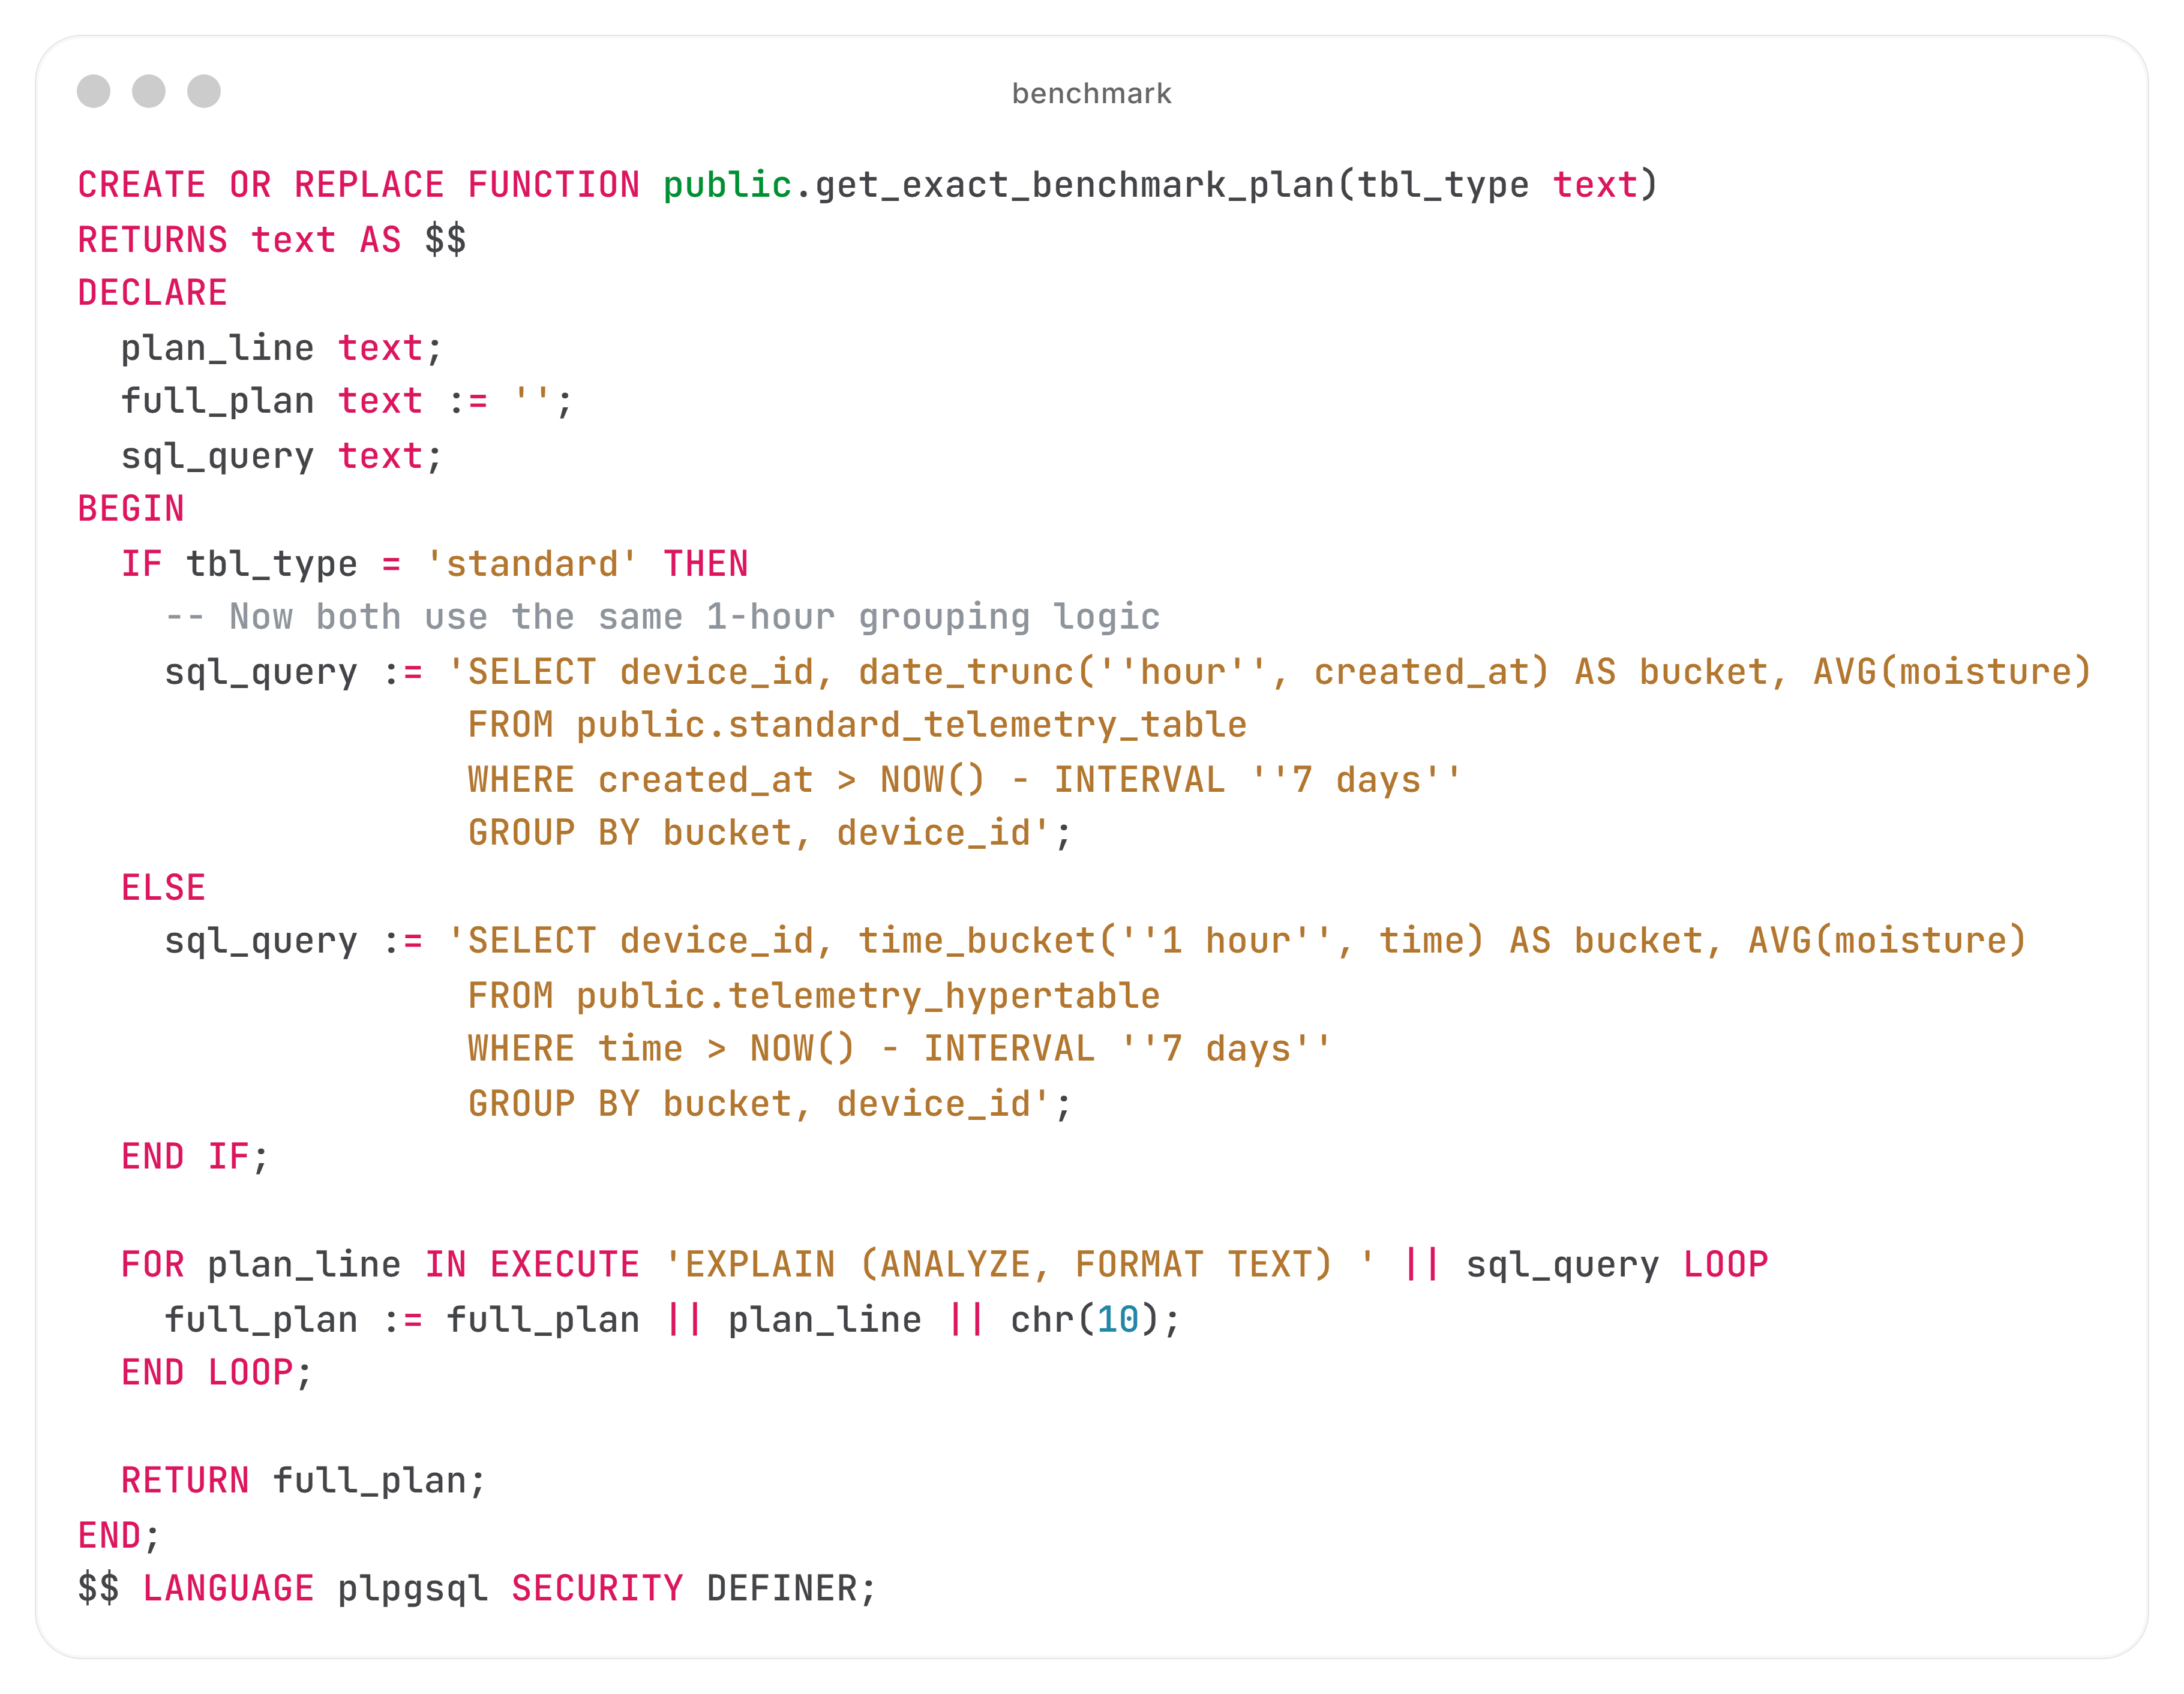
\includegraphics[width=0.8\textwidth]{Abudi/figures/benchmark.png}
    \caption{TimescaleDB aggregation query}
    \label{fig:timescaledb_query}
\end{figure}

The query was run 100 times per benchmarking session, across 10 independent testing runs. The \texttt{EXPLAIN ANALYZE} outputs demonstrated a clear distinction in database behavior: standard PostgreSQL relied entirely on exhaustive Sequential Scans, reading all rows before applying filters. Conversely, the hypertable utilized optimized ChunkAppends combined with Index Scans, ignoring entire sections of irrelevant time data.

Due to this structural advantage, the average query execution time plummeted. The time required was merely 12.4 ms for the hypertable architecture, compared to a lagging 45.7 ms for the plain table. This confirms that implementing TimescaleDB guarantees long-term scalability without heavily inflating cloud computing costs.

\subsubsection{Scenario 2: Infrastructure Resilience (Disaster Recovery Spike)}
Scenario 2 simulates a “Disaster Recovery” event where 50 virtual devices concurrently publish a burst of 10\,k MQTT payloads. The benchmark stresses the middleware’s connection pooling and batch processing, assessing resilience against API rate limits (HTTP 429) and packet loss. Over the 10 runs, the middleware successfully processed 99.8 \% of messages with an average end‑to‑end latency of 28.3 ms.

The results demonstrate that the backend can sustain high‑volume spikes while keeping latency within acceptable bounds, confirming the robustness of the Thin Edge architecture.
